\documentclass{article}

\usepackage[catalan]{babel}
\usepackage[utf8]{inputenc}
\usepackage{fancyhdr}
\usepackage{graphicx}

\pagestyle{fancy}
\fancyhf{}
\rhead{PAP}
\lhead{Designing our own cluster}
\cfoot{Pàgina \thepage}

\setlength{\parindent}{0em}
\setlength{\parskip}{1em}

\begin{document}

\makeatletter
\begin{titlepage}
\thispagestyle{empty}
\begin{center}
	\centering
	\vspace{1cm}
	{\scshape\Large Projectes de laboratori de PAP\par}
	\vspace{0.5cm}
	{\Large Curs 2019/20 (Quadrimestre de primavera)\par}
	\vspace{3cm}
	{\huge\bfseries Designing our own\par HPC-oriented cluster\par}
	\vspace{6cm}
  {\setstretch{0.25}
  {\Large \itshape Rafel-Albert Bros Esqueu\par Andrea Querol de Porras\par Joan Vinyals Ylla-Català\par Pablo Vizcaino Serrano\par}
  }
  \vspace{0.5cm}
  \vfill
	{\large Facultat d'Informàtica de Barcelona\par}
\end{center}
\clearpage
\end{titlepage}


%https://docs.google.com/spreadsheets/d/1h09R-LO8-yKG6tomeKPeug_olNzxpoOcf6uOx5kS5uo/edit?usp=sharing


%https://www.top500.org/news/cavium-releases-thunderx2-arm-processor/
%https://www.ecmwf.int/sites/default/files/elibrary/2018/18590-how-arms-entry-hpc-market-might-affect-meteorological-codes.pdf
%https://store.avantek.co.uk/avantek-64-core-cavium-thunderx2-arm-server-r281-t94.html
%https://store.avantek.co.uk/catalogsearch/result/?q=Thunderx2
%https://www.gigabyte.com/ARM-Server/Marvell-ThunderX2
%https://www.itjungle.com/2018/04/09/counting-the-cost-of-ibm-i-on-power9-entry-systems/
%https://en.wikichip.org/wiki/cavium/thunderx2/cn9980

%Power of CN9980
%https://www.servethehome.com/cavium-thunderx2-review-benchmarks-real-arm-server-option/

\section{Descripció}

La primera qüestió a plantejar-nos ha estat quin seria el processador meś adient. Per a prendre una decisió de la forma més encertada possible, hem cregut oportú elaborar una taula amb diverses possibilitats i comparar les característiques de totes elles. Els principals criteris valorats per a prendre aquesta elecció, tal com es pot veure a la figura \ref{chartCPUs}, han estat els GFlops/Socket, els GFlops/Watt i els GFlops/Dòllar (sent els GFlops normalitzats respecte la mitjana). 

\begin{figure}[h]
    \centering
    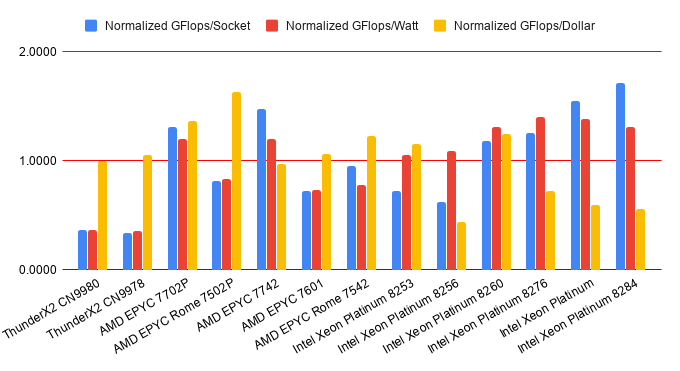
\includegraphics[width=\textwidth]{entregable/fitxers/chartCPU}
    \caption{Comparativa entre les diverses CPUs valorades.}
    \label{chartCPUs}
\end{figure}

Després d'estudiar els resultats, per tenir un major marge de maniobre de cara a decisions futures hem pre-seleccionat dos processadors: l'\textit{AMD EPYC 7702P} \cite{AMDE7702P} i l'\textit{AMD EPYC Rome 7502P} \cite{AMDER7502P}, el primer per mostrar un excel·lent equilibri entre les tres principals característiques estudiades, i el segon per oferir el GFlop més barat sense menystenir excessivament els altres dos aspectes principals.

Seguidament, continuant amb la dinàmica establerta, hem prosseguit a analitzar diversos candidats per a tots i cadascun dels possibles components del clúster. A més, certs elements són opcionals i cal estudiar la seva viabilitat, com per exemple les GPUs. 

No obstant, abans de prosseguir amb els següents aspectes del disseny cal valorar algunes limitacions establertes per la documentació del projecte que seran decisives d'ara endavant. Per exemple, pel que fa a GPUs el nostre disseny ve delimitat per la condició que fins a un màxim del 30\% dels flops del sistema poden provenir de nodes de computació accelerats, és a dir, de nodes amb GPUs. Tanmateix, el nombre màxim de GPUs dependrà de la placa base escollida, que al seu torn depèn del processador que haguem escollit. 

L'espai també serà un problema a tenir en compte: disposem de dos armaris, cadascun d'ells de 42U i, en definitiva, 84U totals. Aquells nodes que contenen una gràfica ocuparan 2U, mentre que aquells que no en tinguin ocuparan 1U. Finalment, cal tenir present la restricció del preu global del sistema en un milió i mig d'euros. 

%Cal anar agafant coses d'aquí sota i anar-ho re-escrivint i col·locant ben maco a sobre:

Cal plantejar a més, un problema. Volem aconseguir el màxim nombre de teraflops satisfent tan les restriccions d'espai de dos armaris (84U) com la del percentatge de teraflops que podem obtenir fruit de l'ús de GPUs. La solució d'aquest escenari ve definit per la tipologia de xarxa així com el nombre de commutadors que emprarem en aquesta xarxa (...), ja que la combinació d'aquests dos factors determinarà el nombre de nodes disponibles en el sisisema.

Entenent que en el nostre cas els nodes que contenen gràfiques ocupen 2U, a diferència dels que no que n'ocupen una, ens convé agrupar les graiques en un subconjunt dels nodes per tenir la major densitat de gràfiques per unitat. El nombre de nodes total ve determinat per la gràfica que utilitzem, el nombre de commutadors utilitzats, el processador que utilitzem, i el nombre de gràfiques que utilitzem. 

Cal entendre que a més commutadors major serà el nombre de nodes [..explicar xarxa..] que podem connectar a la xarxa però, paral·lelament, menor serà el nombre d'unitats que quedaran disponibles pels nodes de computació. Un cop s'hagi delimitat el nombre d'unitats i nodes disponibles, cal cercar la millor combinació possible entre nodes amb GPUs (que ocuparan dues unitats) i nodes lliures de GPUs (que ocuparan una unitat).

A més, entenent que el nostre disseny ve limitat per la condició que un màxim del 30\% dels flops del nostre sistema poden provenir de GPUs, i que el màxim nombre de GPUs varia en funció de la placa base (que ve determinada pel processador utilitzat). Hem explorat totes les configuracions possibles per trobar aquella que ens oferia un major nombre de flops sense sortir de la restricció del preu.

%S'ha de seguir però tinc son, això és tot per avui amics.

\section{Components}

\section{Representació Roofline}

\begin{thebibliography}{}

\bibitem{AMDE7702P} AMD EPYC 7702P: \textit{Newegg Business}, \\
https://www.neweggbusiness.com/product/product.aspx?item=9b-19-113-583
\bibitem{AMDER7502P} AMD EPYC Rome 7502P: \textit{Newegg Business}, \\ https://www.neweggbusiness.com/product/product.aspx?item=9siv1dsa223\\241\&bri=9b-19-113-589

\end{thebibliography}

\end{document}
